\newpage
\section{Aufgabe 1: a}

\subsection{Aufgabenstellung}
Welche Virtualisierungsumgebungen kennen Sie (auch aus anderen Vorlesungen)? Nennen
Sie Vor- und Nachteile. Tipp: die Oracle VirtualBox bietet einen guten Funktionsumfang.
(1 Punkt)

\subsection{Vorbereitung}
Für diese Aufgabe müssen wir erstmal feststellen, welche Virtualisierungsumgebungen wir kennen, welche Funktionalität sie bieten und ob es unterschiedlichen Versionen gibt. 
Wenn wir das getan haben können wir diese miteinander vergleichen.

\subsection{Durchführung}
Wir kennen in unserem Fall zwei verschiedene Virtualisierungsumgebungen. Einmal die VirtualBox von Oracle und die Workstation von VMware.

\begin{figure}[H]
	\begin{minipage}[b]{.5 \linewidth}
		\centering
		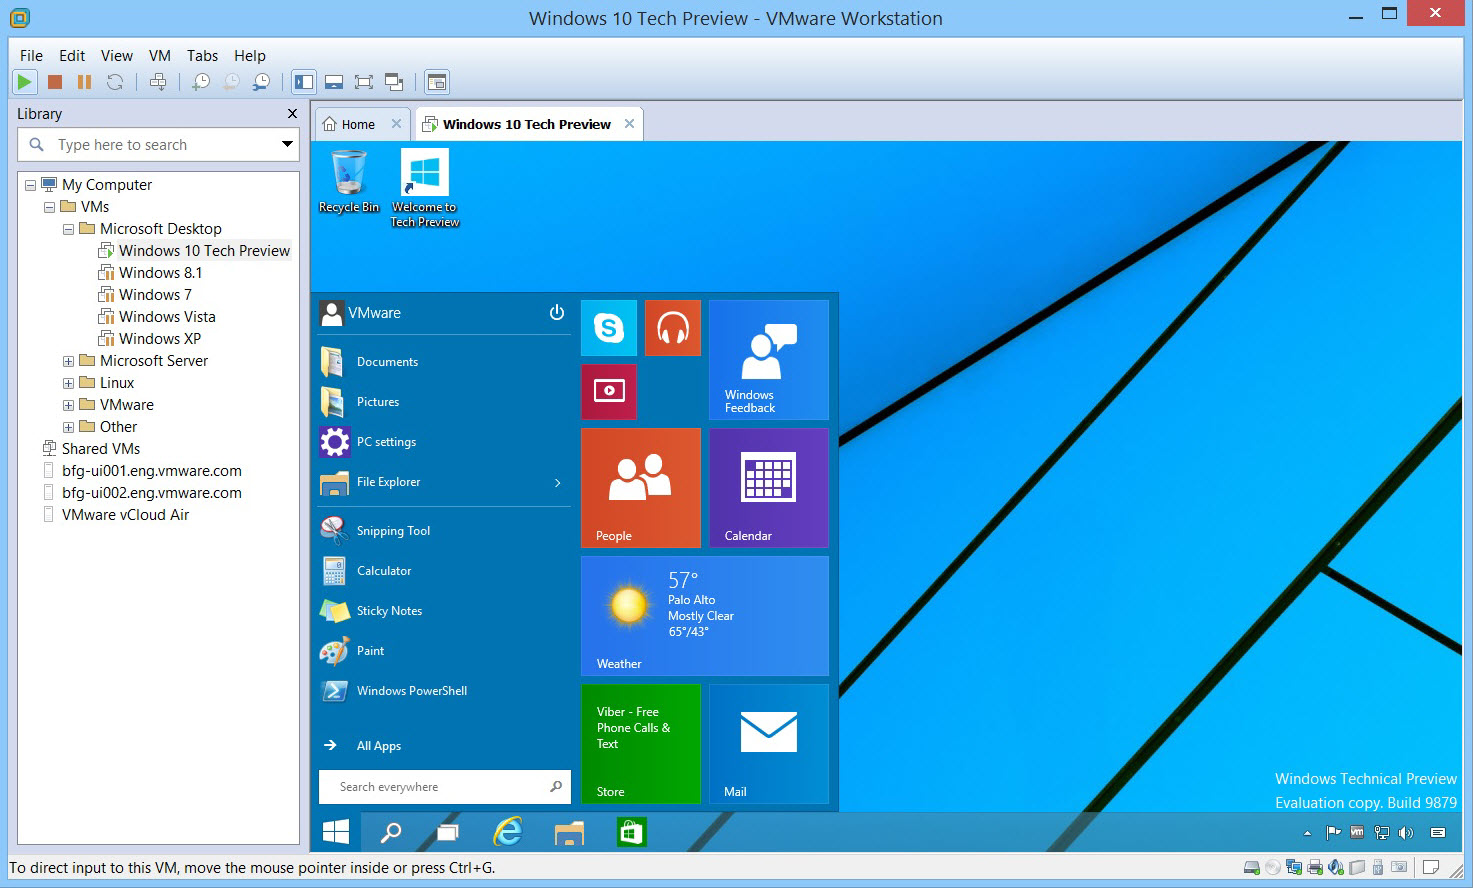
\includegraphics[width=0.8 \linewidth]{images/vmware}
		\subcaption{VMware Workstation \cite{myrhang:2014}} \label{fig:1a}
	\end{minipage}
	\begin{minipage}[b]{.5 \linewidth}
		\centering
		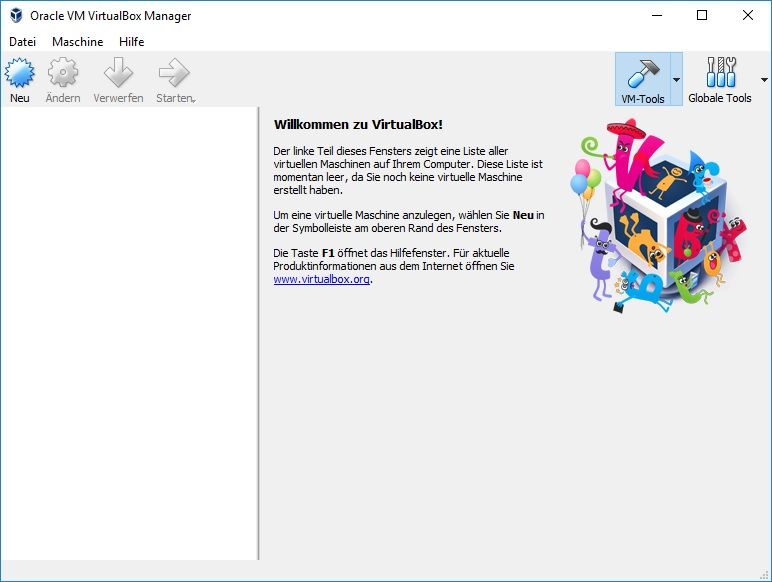
\includegraphics[width=0.8 \linewidth]{images/virtualbox}
		\subcaption{Oracle VirtualBox} \label{fig:1b}
	\end{minipage}
\end{figure}

\subsubsection{VMware Workstation}
VMware Workstation gibt es in zwei verschiedenen Versionen, Player und Pro.
Beide sind von der Grundfunktionalität gleich, die Pro Version bietet ein paar extra Funktionen.  

\begin{table}[H]
	\tablestyle
	\begin{tabular}{llll}
		\toprule
			& Player & Pro \tabularnewline
		\midrule
			\textit{Erstellen von VMs} & \cmark & \cmark \tabularnewline
			\textit{DX10 Unterstützung} & \cmark & \cmark \tabularnewline
			\textit{4K Unterstützung} & \cmark & \cmark \tabularnewline
			\textit{USB 3.0 Unterstützung} & \cmark & \cmark \tabularnewline
			\textit{Verschlüsselte VMs erstellen} &  & \cmark \tabularnewline
			\textit{Verschlüsselte VMs starten} &  & \cmark \tabularnewline
			\textit{Mehrere VMs gleichzeitig starten} &  & \cmark \tabularnewline
			\textit{VMs klonen} &  & \cmark \tabularnewline
			\textit{UEFI Boot} & \cmark & \cmark \tabularnewline
		\bottomrule
	\end{tabular}
	\caption{Vergleich zwischen Workstation Player und Pro \cite{vmware:url}}
\end{table}

\subsubsection{Oracle VirtualBox}
Die VirtualBox von Oracle bietet eine gute Funktionalität, diese ähnelt der von VMware Workstation Pro. Sie kann die grundlegenden Sachen, wie VMs erstellen und bietet ebenfalls USB 3.0 Unterstützung. Die Auflösung ist ohne Treiber auf 800x600 Pixel beschränkt. Hier gibt es nur die kostenfreie Version \cite{virtualbox:url}.

\subsubsection{VirtualBox vs. Workstation Player vs. Workstation Pro}
Wir vergleichen hier die drei Versionen der jeweiligen Anbieter. 

\begin{table}[H]
	\tablestyle
	\begin{tabular}{llll}
		\toprule
			& Oracle VirtualBox & VMware Workstation Player &  VMware Workstation Player \tabularnewline
		\midrule
			\textit{Open Source} & \cmark & & \tabularnewline
			\textit{Kosten} & 0,00 € & 0,00 € & 274,95 € \tabularnewline
			\textit{Snapshots} & \cmark & & \cmark \tabularnewline
			\textit{Drag-N-Drop} & \cmark & \cmark & \cmark \tabularnewline
			\textit{Shared Folder} & \cmark & \cmark & \cmark \tabularnewline
		\bottomrule
	\end{tabular}
\end{table}

\subsection{Fazit}
Alle drei haben ihre Daseinsberechtigung, aber für den End-User und kleine Teams ist die VirtualBox die bessere Wahl, das sie eine ziemlich gute Funktionalität mit sich bringt. Die VMware hat eine bessere Performance, welche man aber mit einem starken Host-System nicht sonderlich merkt.
